% Imporditud: tools/import_eksperimendid.py
% Allikas: Eesti füüsikaolümpiaadi eksperimendi ülesannete
%   kogu (Rael Kalda, 2023), ülesanne Ü104, lahendus L104.
\setAuthor{EFO žürii}
\setRound{lõppvoor}
\setYear{2011}
\setNumber{G E2}
\setDifficulty{3}
\setTopic{elektriahelad}
\setVahendid{kolme väljundklemmiga must kast, multimeeter, mida tohib kasutada milliampermeetrina ja voltmeetrina. Patarei ja multimeetri võib lugeda ideaalseteks}
\setPunktid{12}
\setAllikas{Eksperimendi kogu Ü104, lahendus lk 80}
\setLahendusseis{toores}

\prob{Must kast}
On teada, et mustas kastis paikneb juuresolev skeem. Määrake patarei elektromotoorjõu ja takistite väärtused.
\begin{center}
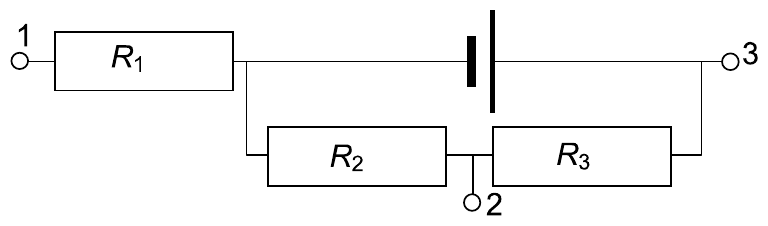
\includegraphics[width=0.55\linewidth]{2011-v3g-ge2-yl.png}
\end{center}

\hint

\solu
Mõõdame pinge U13 kontaktide 1 ja 3 vahel; et voltmeeter on ideaalne, siis takistis $R_1$ puudub vool ja järelikult ka pinge, mistõttu

E = U13.

Mõõdame voolu I13 kontaktide 1 ja 3 vahel; et takistile $R_1$ rakendub patarei kogupinge (ampermeetri takistus on tühine), siis

$R_1$ = E /I13.

Mõõdame voolu I23 kontaktide 2 ja 3 vahel; et ampermeetri takistus on tühiselt väike, siis kogu vool läbib ampermeetrit (vältides takistit $R_3$ ) ja patarei kogupinge rakendub takistile $R_2$, seega

$R_2$ = E /I23.

Mõõdame pinged U12 ja U23, vastavalt kontaktide 1 ja 2 ning 2 ja 3 vahel; et sama vool läbib takisteid $R_2$ ja $R_3$, siis jaguneb patarei pinge neil võrdeliselt takistuste väärtustega. Arvestades, et U12 annab pinge takistil $R_2$ (takistil $R_1$ vool ja pinge puuduvad), saame U12/U23 = $R_2$/$R_3$, millest

$R_3$ = R2U23/U12.
\probend
